\documentclass[12pt,fleqn]{article}\usepackage{../../common}
\begin{document}
Materyel Mekaniği - Hazırlık

Eksenel Yükleme (Uniaxial Loading)

Pek çok problemde kullanılan en temel deformasyon (yamulma, şekil değiştirme)
turu altta görülen tur yüklemedir. Bir demir, ya da plastik çubuk iki kuvvetle
boyu yönünde (tek bir eksende yani) iki tarafa doğru çekilir, bizim
ilgilendiğimiz çubukta seçilen herhangi bir noktanın nereye gittiği, yani
o tek eksendeki deformasyonun ne olduğu.

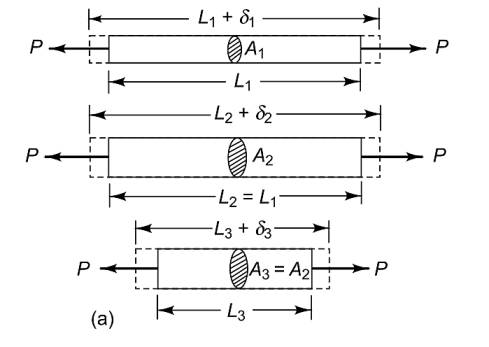
\includegraphics[width=20em]{phy_020_strs_00_01.jpg}

Diyelim ki üstteki her üç çubuk aynı maddeden yapılmış, farklı uzunlukları ve
kalınlıkları var, her çubuğa sıfırdan başlayarak belli seviyelerde yük
uyguluyoruz, ve çubuğun uzunluk değişimi (elongation) $\delta$ değerinin, ki tek
boyuttaki deformasyon budur, ne olduğuna bakıyoruz. Her 1,2,3 çubuğu için $P/A$
ve $\delta/L$ değerlerini grafiklersek çoğunlukla sonuç ya alt soldaki gibi ya
da sağdaki gibi çıkacaktır.

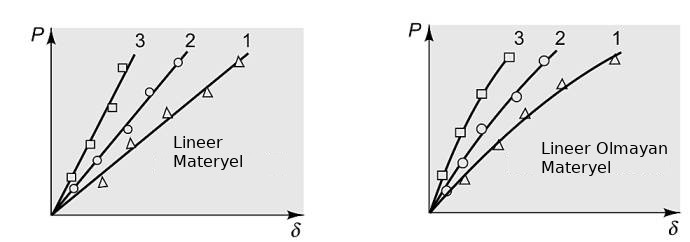
\includegraphics[width=20em]{phy_020_strs_00_02.jpg}

Eğer materyelin eksenel yük ve uzama ilişkisi lineer ise o zaman sonuç soldaki
resim gibi çıkar. Grafiğin eğimine elastiklik genliği (modülüs of elasticity)
adı verilir ve çoğunlukla ona $E$ sembolü verilir. Formülsel olarak belirtirsek,

$$
E = \frac{P/A}{\delta / L}
$$





















\end{document}
